\part{Diskontinuierliche Gruppen}


% ==========
\section{Möbuistransformationen}\label{sec_moebius}

\DB Es sei $X$ ein topologischer Raum und $G$ eine Gruppe von
Homöomorphismen von $X$, die effektiv operiert.
\begin{enumerate}
\item $G$ operiert \emph{diskontinuierlich}\index{diskontinuierlich}\index{Aktion!diskontinuierlich}
in $x\in X$, wenn es
eine offene Umgebung $U$ von $x$ gibt mit $g(U)\cap U=\emptyset$
für alle bis auf endlich viele $g\in G$.
\item $G$ heißt \emph{diskontinuierlich}\index{diskontinuierlich}\index{Gruppe!diskontinuierlich},
wenn es ein $x\in X$ gibt, so dass $G$ in $x$ diskontinuierlich
operiert.
\item Die Menge
\[
\Omega(G) := \{x\in X : G \text{ operiert diskontinuierlich in } x \}
\]
ist eine offene, $G$-invariante Teilmenge von $X$.
Es ist $U\subseteq \Omega(G)$.\index{$\Omega(G)$}
\end{enumerate}

\BSP Diskontinuierliche Gruppen.
\begin{enumerate}
\item Es sei $X=\hat{\CC}:=\PP^1(\CC)$ die
\emph{Riemannsche Zahlenkugel}.\index{Riemannsche Zahlenkugel}\index{$\hat{\CC}$ (Riemmansche Zahlenkugel)}
Es sei $g\in\PGL_2(\CC)$ und $G=\lag g\rag$.
\begin{enumerate}
\item Sei $g$ hyperbolisch.
Dann ist $g$ konjugiert zu $z\mapsto \lambda z$ mit $\lambda\in\CC$,
$|\lambda|>1$.
Setze $U:=\{z\in\CC : 1<|z|<|\lambda| \}$.
\begin{center}
	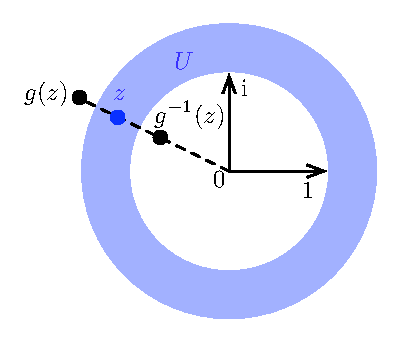
\includegraphics{UinC}
\end{center}
Für $z\in U$ und $n\in\ZZ$ ist $g^n(z)=\lambda^n z$,
also
\[
|g^n(z)|=|\lambda|^n |z|=
\left\{
\begin{matrix}
>|\lambda|, & n\geq 1 \\
< 1, & n\leq -1 \\
|z|, & n=0
\end{matrix}
\right..
\]
Also ist $g^n(U)\cap U=\emptyset$ für $n\neq 0$.
Damit ist $G$ diskontinuierlich und es ist
$\Omega(G)=\hat{\CC}\backslash\{0,\infty\}$.
\item ..
\item ...
\end{enumerate}
\end{enumerate}